\documentclass{standalone}
\usepackage{pgfplots}
\usepackage{amsmath}
\usetikzlibrary{decorations.markings}
\pgfplotsset{compat=newest}

%%%% Differential /x^2stem %%%%%
\def\xdot{(-y+x^2-y^2)/(1+2*y)^2}
\def\ydot{x/(1+2*y)}
%%%%%%%%%%%%%%%%%%%%%%%%%%%%%%

%%%% First integral %%%%
\def\firstint{(x^2+y^2)/(1+2*y)}
%%%%%%%%%%%%%%%%%%%%%%%%

\def\eps{0.05}

\begin{document}
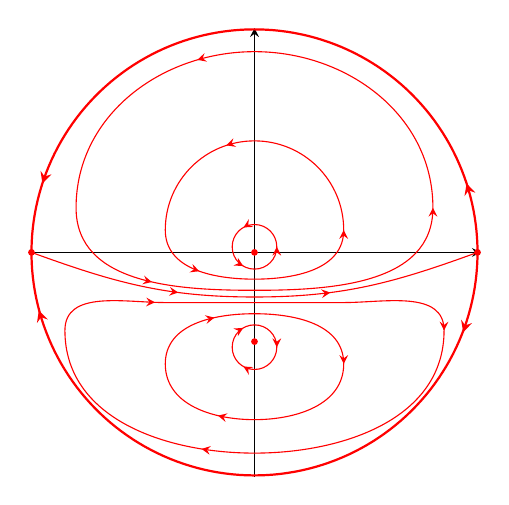
\begin{tikzpicture}[every node/.style={scale=0.85},decorated arrow/.style={
        postaction={
            decorate,
            decoration={
                markings,
                mark=at position 0.333 with {\arrow[red]{stealth}},
                mark=at position 0.666 with {\arrow[red]{stealth}}}}
      },decorated arrowcirc/.style={
        postaction={
            decorate,
            decoration={
                markings,
                mark=at position 0 with {\arrow[red]{stealth}},
                mark=at position 0.333 with {\arrow[red]{stealth}},
                mark=at position 0.666 with {\arrow[red]{stealth}},
              }}
      },decorated arrowcircout/.style={
        postaction={
            decorate,
            decoration={
                markings,
                mark=at position \eps with {\arrow[red]{stealth}},
                mark=at position 0.5-\eps with {\arrow[red]{stealth}},
                mark=at position 0.5+\eps with {\arrow[red]{stealth[reversed]}},
                mark=at position 1-\eps with {\arrow[red]{stealth[reversed]}},
              }}
      }]
  \begin{axis}[
      axis lines=middle,
      xmin=-1.0145,xmax=1.0145,
      ymin=-1.0051, ymax=1.0051,
      % xlabel = {$x$},
      % ylabel = {$y$},
      xtick={0},
      ytick={0},
      axis equal image,
      trig format plots=rad,
      %colormap/vidris,
    ]
    \def\y{-0.4};
    \coordinate (A1) at (0,0);
    \coordinate (L) at (0,{\y/2});
    \coordinate (A2) at (0,{\y});
    \coordinate (B1) at (-1,0);
    \coordinate (B2) at (1,0);

    \def\xmax{\pgfkeysvalueof{/pgfplots/xmax}}
    \def\xmin{\pgfkeysvalueof{/pgfplots/xmin}}
    \def\ymax{\pgfkeysvalueof{/pgfplots/ymax}}
    \def\ymin{\pgfkeysvalueof{/pgfplots/ymin}}
    \addplot[thin,mark=*,only marks, mark size=1pt,red] coordinates {
        (0,0) (0,{\y}) (-1,0) (1,0)
      };
    \addplot [
      samples=200,
      domain=0:2*pi,
      red,
      thick,
      decorated arrowcircout,
    ] ({cos(x)},{sin(x)});
    \draw[red,decorated arrow] (B1) to[out=-20,in=180] (L) to[out=0,in={180+20}] (B2); % invariant line
    % Above cercles
    \draw[red,decorated arrowcirc] (0.1,0+0.025) to[out=90,in=0] (0,0.1+0.025) to[out=180,in=90] (-0.1,0+0.025) to[out=-90,in=180] (0,-0.1+0.025) to[out=0,in=-90] (0.1,0+0.025);
    \draw[red,decorated arrowcirc] (0.4,0.1) to[out=90,in=0] (0,0.5) to[out=180,in=90] (-0.4,0.1) to[out=-90,in=180] (0,-0.1-0.02) to[out=0,in=-90] (0.4,0.1);
    \draw[red,decorated arrowcirc] (0.8,0.2) to[out=90,in=0] (0,0.9) to[out=180,in=90] (-0.8,0.2) to[out=-90,in=180] (0,-0.1-0.07) to[out=0,in=-90] (0.8,0.2);
    % Below cercles
    \draw[red,decorated arrowcirc] (0.1,\y-0.025) to[out=-90,in=0] (0,\y-0.1-0.025) to[out=180,in=-90] (-0.1,\y-0.025) to[out=90,in=180] (0,\y+0.1-0.025) to[out=0,in=90] (0.1,\y-0.025);
    \draw[red,decorated arrowcirc] (0.4,-0.5) to[out=-90,in=0] (0,-0.75) to[out=180,in=-90] (-0.4,-0.5) to[out=90,in=180] (0,-0.2-0.075) to[out=0,in=90] (0.4,-0.5);
    \draw[red,decorated arrowcirc] (0.85,-0.35) to[out=-90,in=0] (0,-0.9) to[out=180,in=-90] (-0.85,-0.35) to[out=90,in=180] (-0.4,-0.225) to[out=0,in=180] (0,-0.2-0.025) to[out=0,in=180] (0.4,-0.225) to[out=0,in=90] (0.85,-0.35);
    %\draw[red,decorated arrowcirc] (B1) to[out=-20,in=180] (L) to[out=0,in={180+20}] (B2);

  \end{axis}
  % \begin{axis}[
  %     grid=both,
  %     xmin=-1,xmax=1,
  %     ymin=-1,ymax=1,
  %     %zmin=0,zmax=2500,
  %     %tick label style={font=\tiny},
  %     %xtick={-2,-1.5,...,2},
  %     %ytick={-1,-0.5,...,3},
  %     %ztick={0,500,...,2500},
  %     %view={0}{90},
  %     xlabel={$x$}, ylabel={$y$},
  %     axis equal image,
  %     % colormap/jet, point meta=ln(z+1),
  %   ]
  %   % \addplot3[surf,shader=flat] {sqrt(1-x^2-y^2)};
  %   % \addplot3[surf,domain=-1.5:1.5, y domain=-1.5:1.5] {sqrt(1-x^2-y^2)};
  %   % \addplot3 [
  %   %   surf,
  %   %   z buffer=sort,
  %   %   % colormap={periodic}{
  %   %   %     color=(color_blue1)
  %   %   %     color=(color_blue2)
  %   %   %     color=(color_blue3)
  %   %   %     color=(color_blue2)
  %   %   %     color=(color_blue1)
  %   %   %   },
  %   %   domain=0:180, domain y=0:360,
  %   %   samples=20, samples y=20,
  %   %   variable=\u, variable y=\v,
  %   %   point meta=u,
  %   % ] (
  %   % {sin(u) * cos(v)},
  %   % {sin(u) * sin(v)},
  %   % {cos(u)}
  %   % );
  %   \addplot3 [
  %     blue,-stealth,
  %     domain=0:1, domain y=0:360,
  %     samples=5, samples y=10,
  %     variable=\r, variable y=\o,
  %     quiver,quiver/.cd,
  %     % u={-(x^2*(2*y + 1)*y/(x^2 + y^2 + 1) + (x^2 - y^2 - y)*(x/sqrt(x^2 + y^2 + 1) - 1))/sqrt(x^2 + y^2 + 1)},
  %     % v={(x*(2*y + 1)*(y^2/(x^2 + y^2 + 1) - 1) - (x^2 - y^2 - y)*x*y/(x^2 + y^2 + 1))/sqrt(x^2 + y^2 + 1)},
  %     % w={-(x*(2*y + 1)*y/sqrt(x^2 + y^2 + 1) + (x^2 - y^2 - y)*x/sqrt(x^2 + y^2 + 1))/(x^2 + y^2 + 1)},
  %     % u={-((2*cos(o)^3 - cos(o))*r^5 - r^4*cos(o)*sin(o) + (2*cos(o)^3 - cos(o))*r^3 - r^2*cos(o)*sin(o) - ((2*cos(o)^4 - 1)*r^4 - (cos(o)^2 + 1)*r^3*sin(o) + (2*cos(o)^2 - 1)*r^2 - r*sin(o))*sqrt(r^2 + 1))/(r^4 + 2*r^2 + 1)},
  %     % v={-((4*cos(o)^3 - cos(o))*r^4*sin(o) + (2*cos(o)^3 - cos(o))*r^3 + 2*r^2*cos(o)*sin(o) + r*cos(o))*sqrt(r^2 + 1)/(r^4 + 2*r^2 + 1)},
  %     % w={-sqrt(r^2 + 1)*r^3*cos(o)/(r^4 + 2*r^2 + 1)},
  %     u={r*cos(o)/sqrt(r^2+1)},
  %     v={r*sin(o)/sqrt(r^2+1)},
  %     w={0},
  %     scale arrows=0.1,
  %   ] (
  %   % {x/sqrt(x^2+y^2+1)},
  %   % {y/sqrt(x^2+y^2+1)},
  %   % {1/sqrt(x^2+y^2+1)}
  %   {r*cos(o)/sqrt(r^2+1)},
  %   {r*sin(o)/sqrt(r^2+1)},
  %   {1/sqrt(r^2+1)}
  %   );

  %\end{axis}
\end{tikzpicture}
\end{document}